\clearpage
\section{\texorpdfstring{Untersuchung einer $\text{TiSe}_2$-Probe}{Untersuchung einer TiSe2-Probe}}
\label{sec:thijs2}

Dieser Abschnitt beschäftigt sich mit der Suche nach einem Zustand im Leitungsband, welcher sich nach einer temperaturbedingten Phasenänderung in einer $\text{TiSe}_2$-Probe ergeben sollte.
Dafür wird die Probe gekühlt und ein inverses Photoemissionspektrum aufgenommen.
Die unbesetzte elektronische Struktur wird dabei in normaler und CDW Phase untersucht. % ich verstehe nur das "im Allgemeinen" nicht, same; daher weg
Das schließt verschiedene Zustände ein wie z.B. auch das Auftreten eines Bildladungszustandes nahe der Fermi-Energie.

\subsection{Theoretische Grundlagen}
\label{sec:theo1}

Zum Verständnis des hier dargestellten Versuchaufbaus sind Wissen über inverse Photoemission (IPE), Beugung niederenergetischer Elektronen an Oberflächen (engl. LEED) und die zu verwendende $\text{TiSe}_2$-Probe notwendig.
% irgendwie unnötig der Satz, oder? Das gilt doch einfach immer für alle Kapitel in der Theorie, ansonsten wären sie ja überflüssig. w/e, aber halt unnötig.
% -> Ja. Irgend 1 Betreuer meinte mal, dass unter jeden Abschnitt iwas stehen sollte, damit da nicht 4, 4.1, 4.1.1 untereinander gestacked sind. War sehr pingelig der Mensch, aber seitdem habe ich das in der Regel gemacht. Beim letzten Bericht nicht, weil ich konsistent mit deinem geblieben bin. Wenn's dich juckt, kannst du den rausnehmen.

\subsubsection{Inverse Photoemission und Proportionalitätszählrohr}

\begin{figure}[!ht]
    \centering
    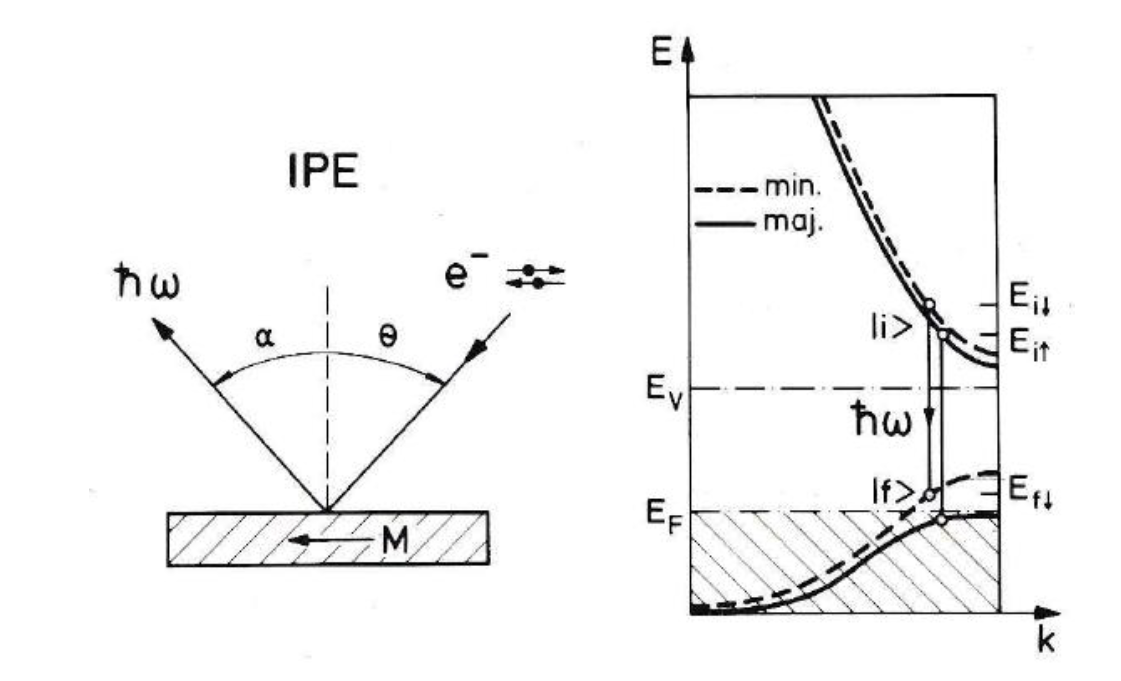
\includegraphics[width=0.5\textwidth]{img/ipe_theo.png}
    \caption{Schematische Darstellung der inversen Photoemission.\cite{donath}}
    \label{fig_ipe_theo}
\end{figure}
Wie der Name impliziert, handelt es sich bei der inversen Photoemission um einen umgekehrten Photoeffekt.
Zur Veranschaulichung dient \cref{fig_ipe_theo}.
Ein niederenergetischer Elektronenstrahl ($<\SI{20}{\electronvolt}$ \cite{wiki_ipe}; hier ca. \SI{6}{\electronvolt}) wird dazu auf eine Probe gerichtet.
Es handelt sich um eine oberflächensensitive Methode, da die Elektronen aufgrund ihrer geringen Energie nur wenige Atomlagen tief eindringen.
Die Elektronen des Elektronenstrahls koppeln an Niveaus oberhalb der Vakuum-Energie an und fallen dann in unbesetzte Zustände oberhalb der Fermi-Energie.
Durch Rekombination entstehen Photonen mit einer für den Übergang charakteristischen Energie $\hbar\omega$.
Daher können aus der Photonenenergie Rückschlüsse auf die Bandstruktur des Materials gezogen werden.
Um die Photonen zu detektieren, werden für diesen Versuch Proportionalitätszählrohre verwendet.
Allgemein für Zählrohre ist, dass ionisierende Strahlung (hier die Photonen) das Zählgas ionisiert und dabei Elektronen frei werden.
Diese Elektronen werden über ein elektrisches Feld in Richtung Anode beschleunigt.
Für das Proportionalitätszählrohr ist die angelegte Spannung so gewählt, dass sich die Zählrohrcharakteristik im Proportionalbereich liegt.
Das bedeutet, dass die freigesetzten Elektronen stark genug beschleunigt werden, um durch Stöße mit dem Zählgas weitere Elektronen herauszulösen, welche dann ebenfalls in Richtung Anode beschleunigt werden.
Deren Gesamtzahl der Elektronen in dieser Lawine ist proportional zur Energie des eingefangenen Photons, sodass das Integral über den an der Anode gemessenen Strom, also die getrennte Ladung, ebenfalls proportional zur Photonenenergie ist.

\subsubsection{Beugung niederenergetischer Elektronen an Oberflächen}

\begin{figure}[!ht]
    \centering
    \includegraphics[width=0.5\textwidth]{img/leed_theo.png}
    \caption{Schematische Darstellung der Beugung niederenergetischer Elektronen an Oberflächen.\cite{leed_theo}}
    \label{fig_leed_theo}
\end{figure}

Ähnlich wie bei der IPE wird ein niederenergetischer Elektronenstrahl auf die Probe gerichtet.
Hierbei liegen die Energien jedoch in einer Größenordnung von \SI{100}{\electronvolt}\cite{wiki_leed}.
Die an der Probe gebeugten Elektronen treffen auf einen LEED-Schirm, welcher aus mehreren Gittern und einem Leuchtschirm besteht, wie in \cref{fig_leed_theo} zu erkennen ist.
Die Gitter sind elektrisch so geschaltet, dass zwischen Probe und erstem Gitter ein feldfreier Raum entsteht, aber innerhalb der Gitter inelastisch gestreute Elektronen größtenteils ausgesondert werden und die verbleibenden, gebeugten Elektronen auf den Schirm beschleunigt werden.
Aus dem Interferenzmuster der gebeugten Elektronenstrahlen, welches sich auf dem Leuchtschirm aufzeichnet, kann die Gitterstruktur der Probe entnommen werden.
Anzumerken ist, dass es sich bei dem Interferenzmuster nicht direkt um die Gitterstruktur handelt, sondern um die Punkte im $k$-Raum, welche die Laue-Bedingung für konstruktive Interferenz erfüllen.

\subsubsection{\texorpdfstring{Die $\text{TiSe}_2$-Probe}{Die TiSe2-Probe}}

Bei $\text{TiSe}_2$ handelt es sich um ein Übergangsmetall-Dichalkogenid (engl. TMDC).
Da TMDC-Monolagen kein Inversionszentrum besitzen, ändert sich die elektronische Struktur markant beim Übergang vom Kristall zur Monolage.
Damit spalten sich die K-Punkte der hexagonalen Struktur des reziproken Gitters zu spin-polarisiertem K$^{-}$- und K$^{+}$-Tälern auf. %theoretisch höufig \bar{K} für reziprok, aber geht wohl auch so. In der Literatur sehe ich iwie immer mal das eine, mal das andere \shrug
Besonders an $\text{TiSe}_2$-Monolagen ist, dass sogenannte Ladungsdichtewellen (engl. CDW) zweier benachbarter Atome bei Temperaturen unter \SI{200}{\kelvin} zusammenziehen und dazu führen, dass sich die Brillouinzone rückfaltet.
Allgemein lassen sich Ladungsdichtewellen durch die kollektiven Leitungseigenschaften im Grundzustand beschreiben.%hier fehlt kein Satz, was CDWs sind.
Durch die Halbierung der Brillouinzone wird aus dem vorherigen M-Punkt bereits der nächste $\Gamma$-Punkt, weswegen dort, wo vorher keine Zustände verzeichnet wurden, nun welche mit Verfahren wie der Photonenemissions-Spektroskopie sichtbar werden, wie z. B. in \cite{tise_pe}.
Analog zu neuen Valenzbandzuständen sind auch neue Leitungsbandzustände zu erwarten, welche mit IPE erprobt werden können. % erprobt oder geprobt?


\subsection{Experimenteller Aufbau}

Bei dem Versuchsaufbau handelt es sich um einen Eigenbau der AG Donath.
Es handelt sich um ein Gerät mit drei Ebenen für verschiedene Anwendungen.
Eine Darstellung der verschiedenen Ebenen ist \cref{fig_ipe_setup} zu entnehmen.
\begin{figure}[!ht]
    \centering
    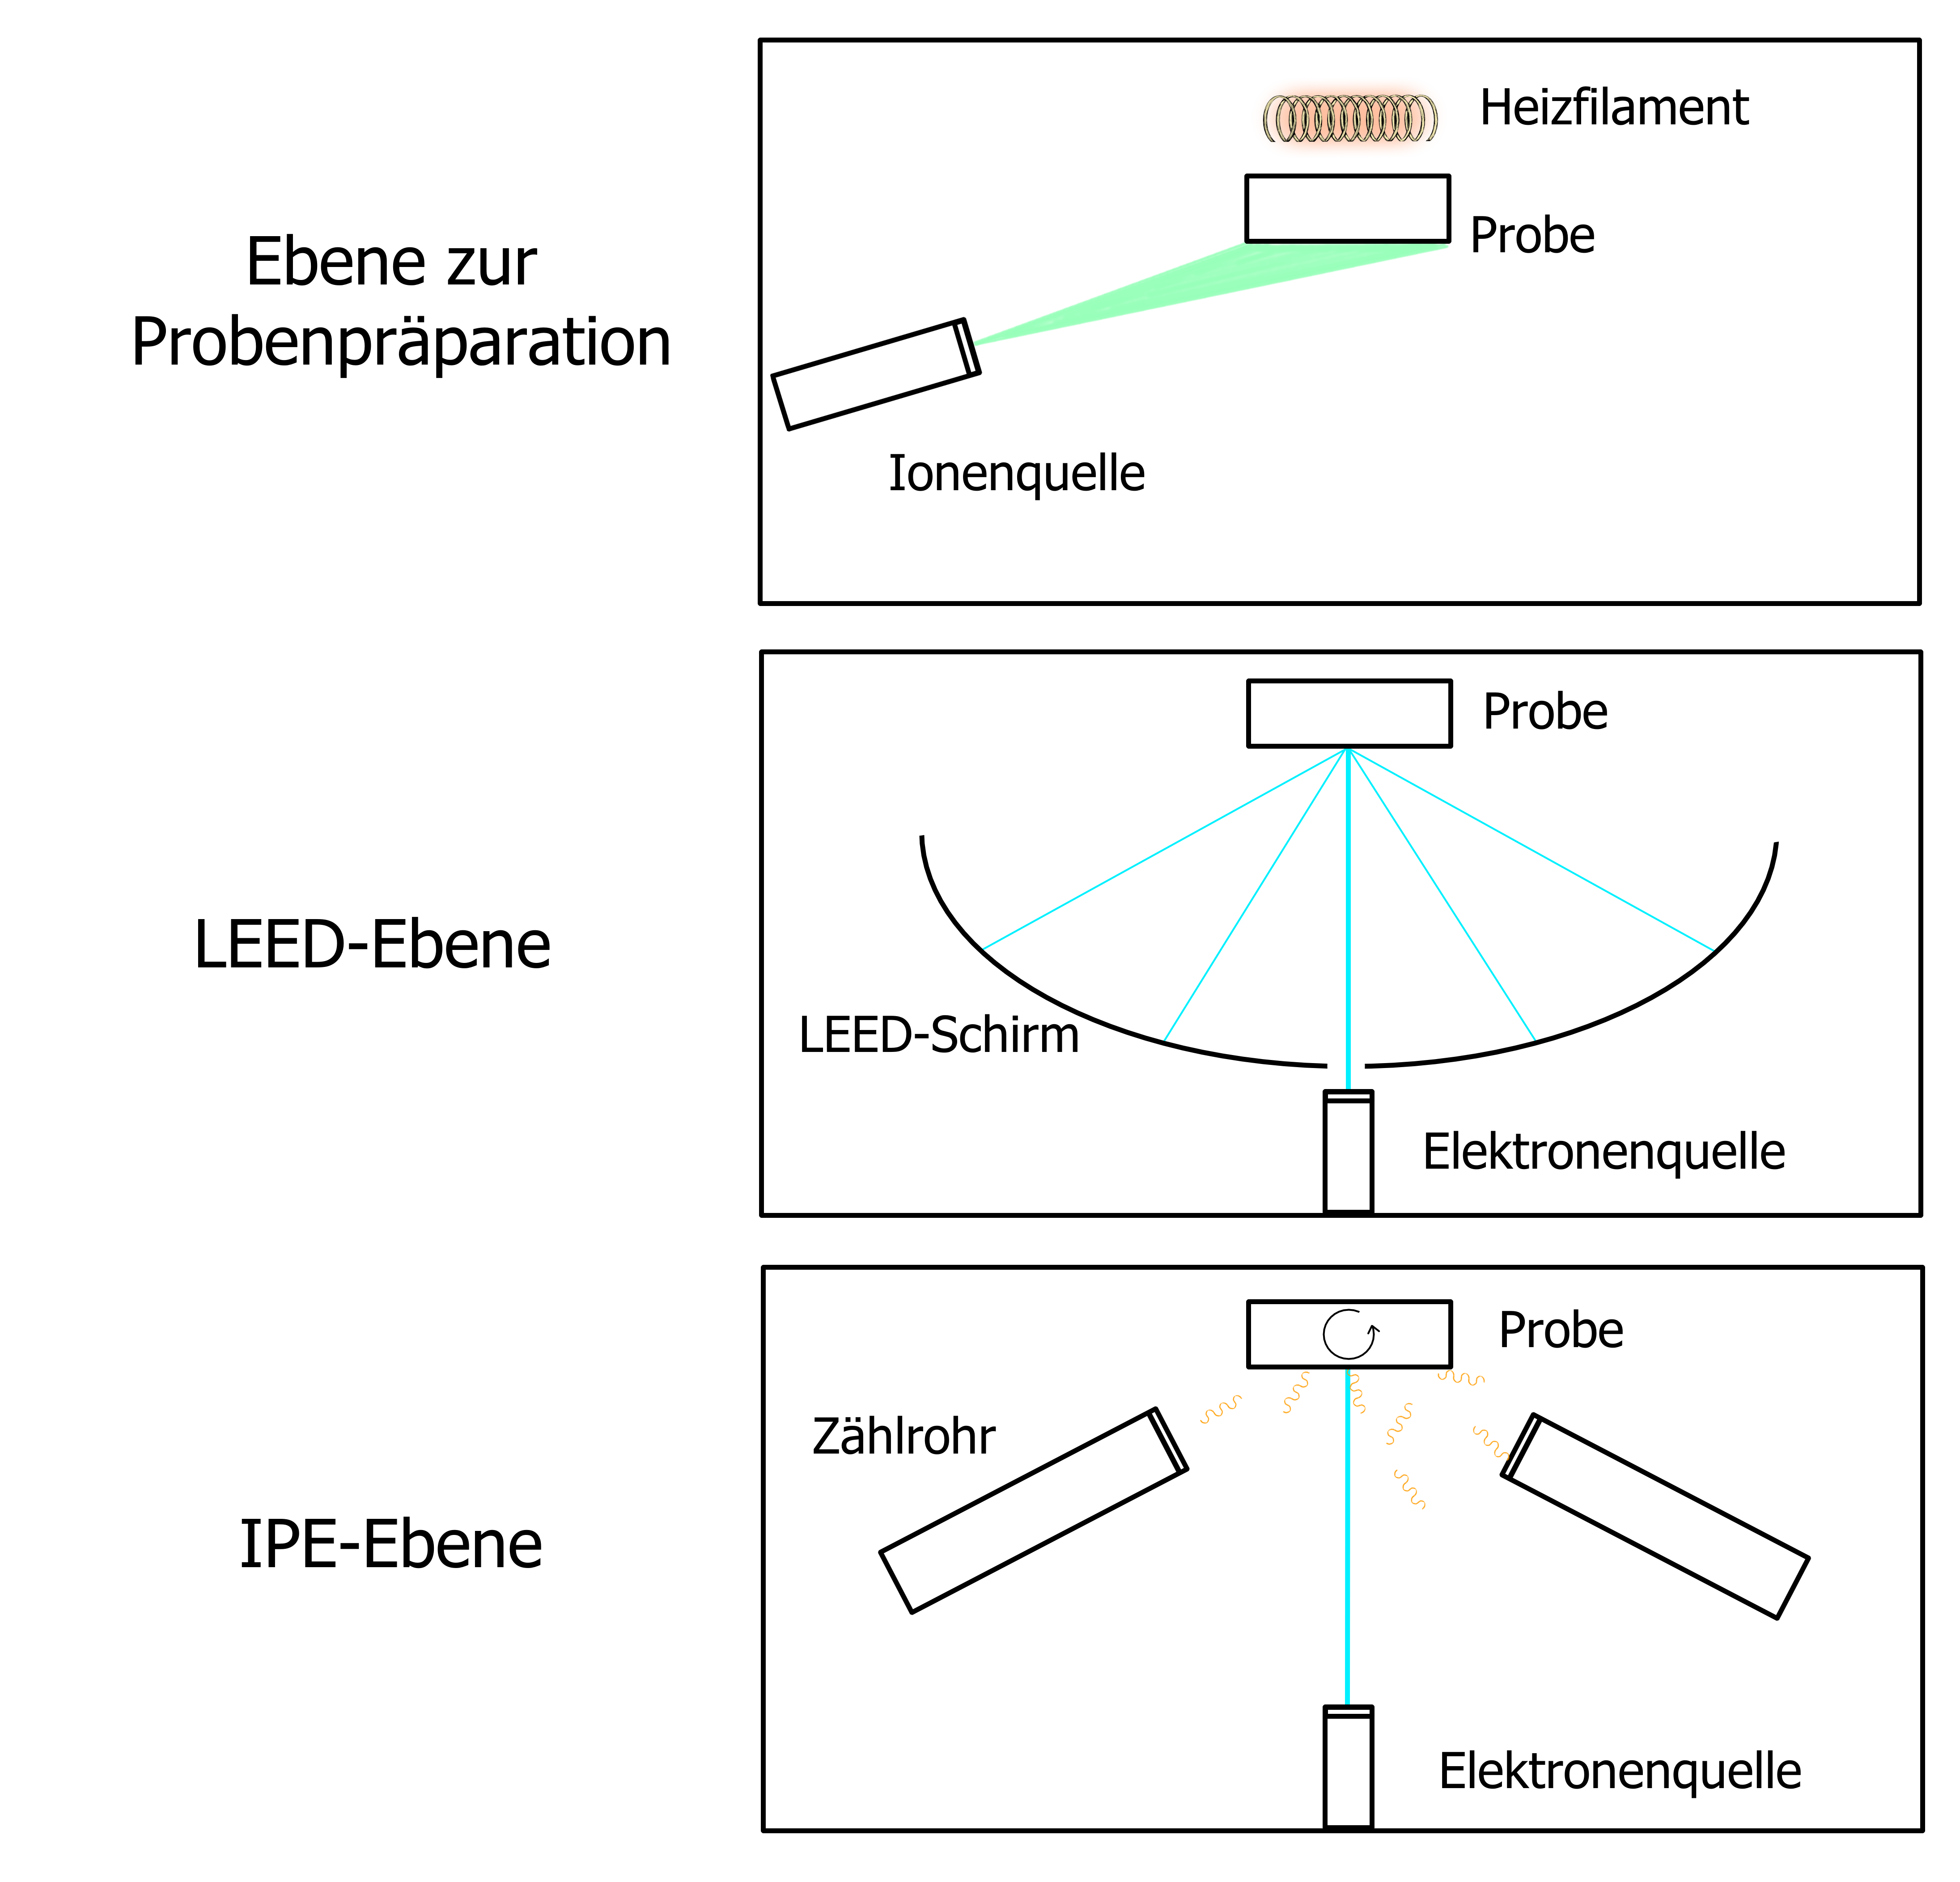
\includegraphics[width=0.75\textwidth]{img/setup1.png}
    \caption{Schematische Darstellung der verschiedenen Ebenen des Versuchaufbaus.
    Nicht dargestellt sind die Vakuumpumpen, der Gaseinlass für die Ionenquelle, der Probeneinlass und der Manipulator über den die Probe zwischen den Ebenen wechseln kann. Zudem liegt noch eine Kühlung für den Manipulator vor.}
    \label{fig_ipe_setup}
\end{figure}
Da alle Anwendungen Hochvakuum benötigen, sind zusätzlich mehrere Vakuumpumpen (Vorpumpe, Turbopumpe) an das Gerät angeschlossen.
Die Probe wird über eine Einschleusungsstange an einem zentralen Manipulator befestigt und kann dann zu den unterschiedlichen Ebenen geschoben werden.
Hier verhalten sich die LEED- und IPE-Ebene wie in \cref{sec:theo1} beschrieben.
Um verschiedene Detektionswinkel zu beobachten, werden für die IPE zwei Zählrohre verwendet und es besteht die Möglichkeit die Orientierung der Probenoberfläche über den Manipulator anzupassen.
In der Ebene zur Probenpräparation befinden sich eine Heizspule, um Oberflächen zu glätten oder Schutzschichten abzudampfen und eine Ionenquelle zum Sputtern.
Das Sputtern dient dazu, Oberflächenverunreinigungen zu bereinigien, weswegen die Einstrahlung nahezu parallel erfolgt.

\subsection{Durchführung und Diskussion}

Bevor eine IPE-Messung für die $\text{TiSe}_2$-Probe durchgeführt werden kann, ist es notwendig eine Kalibration der Messinstrumente durchzuführen.
Zu diesem Zweck wird ein Kupferkristall verwendet, da er in einer (111)-Orientierung und einem Einstrahlwinkel von \SI{12}{\degree} einen Oberflächenzustand bei ca. \SI{6}{\electronvolt} besitzt, welcher bei \SI{0}{\degree} verschwindet.
Um die Kalibrationsmessung durchzuführen, ist es zunächst nötig, die Kupferprobe zu präparieren.
Dafür wird es auf dem Manipulator angebracht und in die Präparationsebene gefahren.
Zunächst wird die Oberfläche mit Argonionen gesputtert, um Verunreinigungen zu entfernen.
Da dies eine sehr unebene Oberfläche zurücklässt wird die Probe anschließend erhitzt, um die Oberfläche ausheilen zu lassen.
Das Heizen erfolgt von der Rückseite der Probe, um die Oberfläche nicht zu beschädigen und währenddessen wird der Manipulator wird mit Stickstoff gekühlt, damit von ihm weniger Verunreinigungen in die Kammer desorbieren.

\begin{figure}[!ht]
    \centering
    \begin{subfigure}{0.495\textwidth}
        \centering
        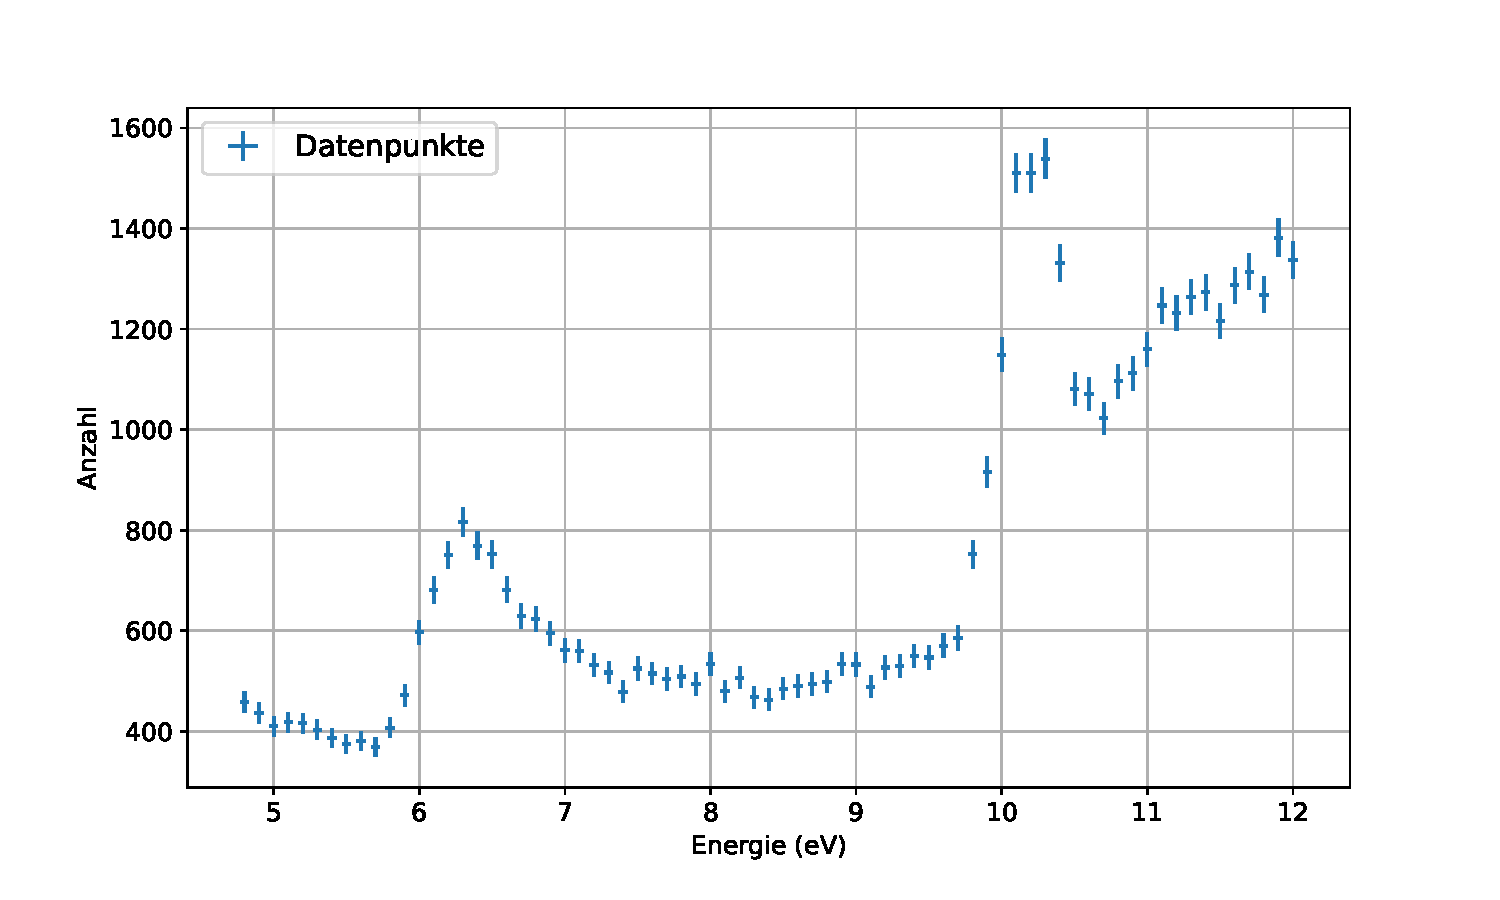
\includegraphics[width=1.1\textwidth]{plots/Cu_0.pdf}
    \caption{}
    \end{subfigure}
    \begin{subfigure}{0.495\textwidth}
        \centering
        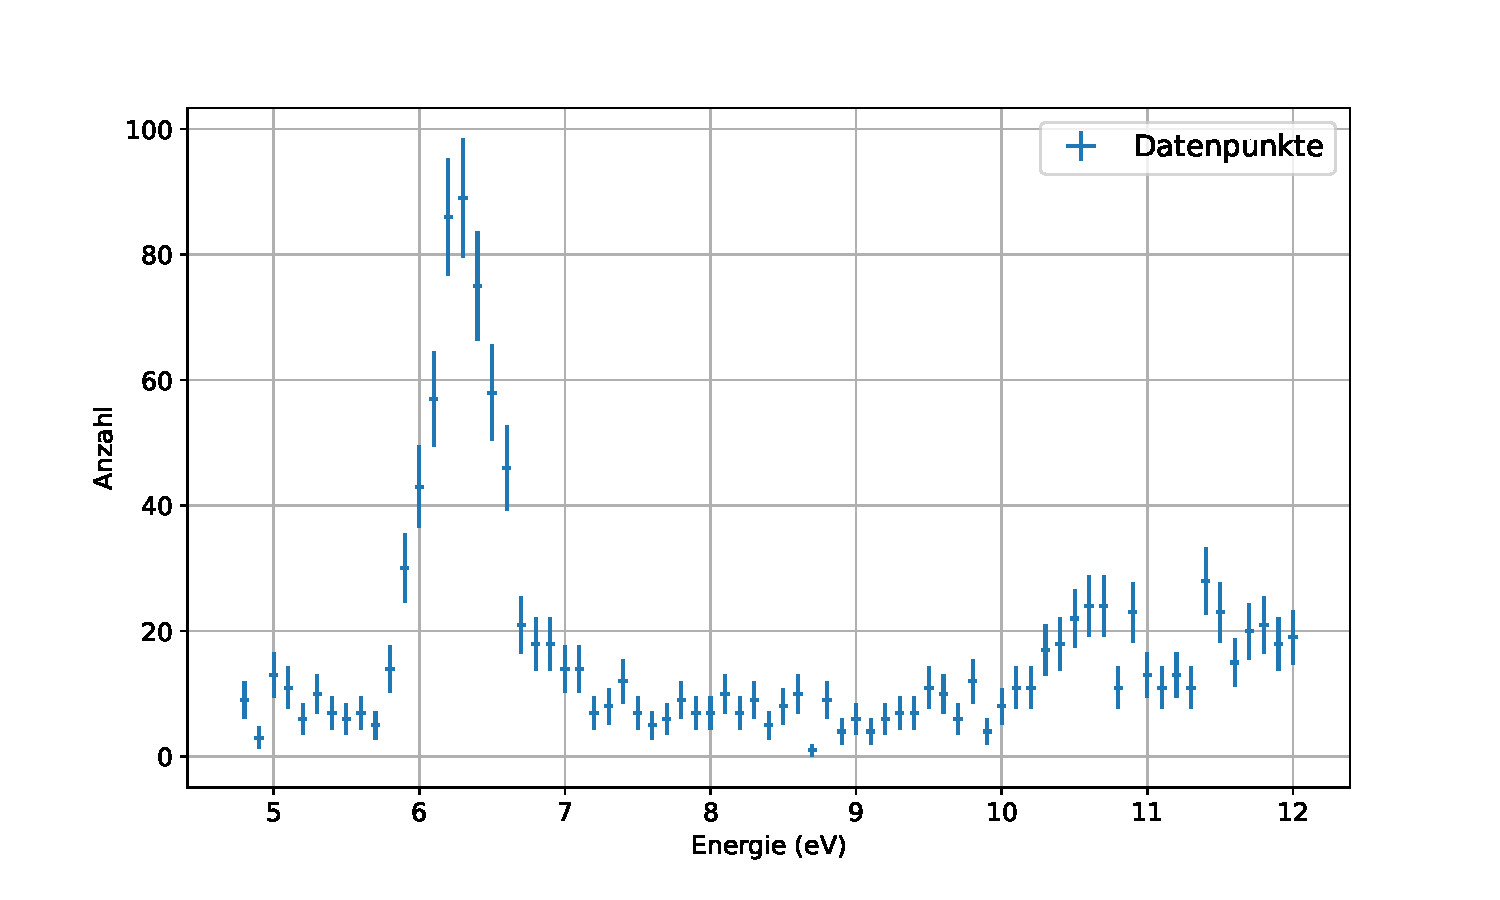
\includegraphics[width=1.1\textwidth]{plots/Cu_12.pdf}
        \caption{}
    \end{subfigure}
    \caption{IPE-Spektren von Kupfer (111) bei (a) \SI{0}{\degree} und (b) \SI{12}{\degree} Einstrahlwinkel.}
    \label{fig_Cu_kal}
\end{figure}
Die anschließend aufgenommen Kalibrationsspektren für \SI{0}{\degree} und \SI{12}{\degree} sind in \cref{fig_Cu_kal} dargestellt.
Aus dem Verhältnis zum Rauschhintergrund lässt sich der Oberflächenzustand bei \SI{12}{\degree} direkt zu entnehmen.
Da dies bereits nach wenigen Messdurchläufen hervorging, wurden dort deutlich weniger Datenpunkte aufgenommen als bei der \SI{0}{\degree} Messung.
Bei letzterer ist erkennbar, dass der Oberflächenzustand nicht verschwindet, aber ein deutlich kleineres Verhältnis zum Hintergrundrauschen aufweist.
Vermutlich lag keine optimale Probenpräparation vor und es könnten sich über den Messzeitraum Verunreinigungen auf der Probenoberfläche angesammelt haben.
Auch die Winkeldivergenz des Elektronenstrahls kann zu groß gewesen sein.
Für die Größe der Unsicherheit der Anzahl wird $\sqrt{n}$ für die Anzahl $n$ verwendet und für die Energieunsicherheit eine stetige Gleichverteilung über den mittleren Abstand der Datenpunkte.

\

\begin{figure}[!ht]
    \centering
    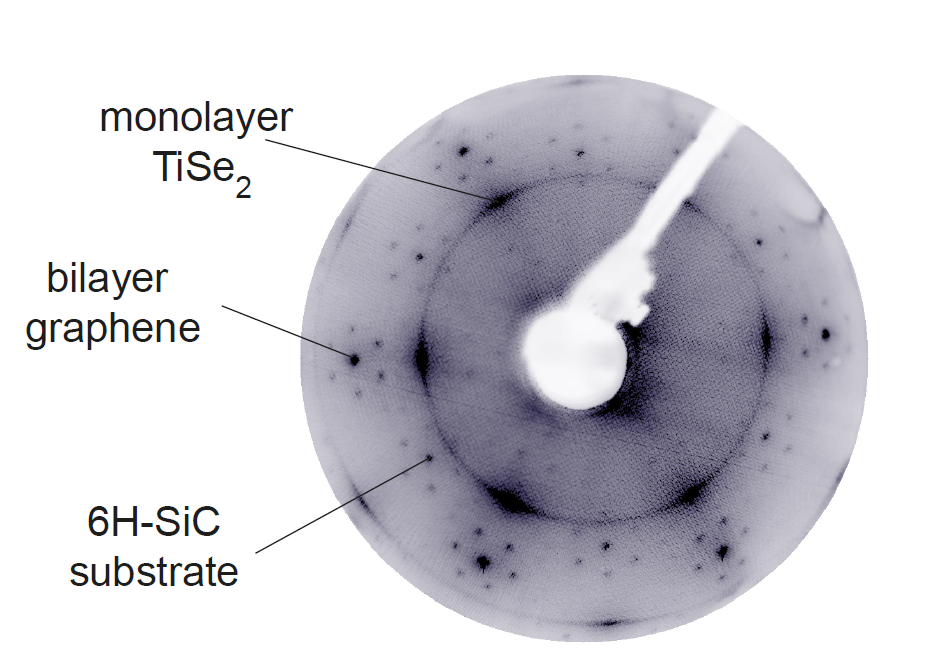
\includegraphics[width=0.5\textwidth]{img/TiSe2LEED}
    \caption{LEED Aufnahme einer $\text{TiSe}_2$-Probe von \cite{leed_sample} zum Vergleich.}
    \label{fig_leed_sample}
\end{figure}
Vor der Messung der $\text{TiSe}_2$-Probe ist jedoch ein weiterer Schritt notwendig, da sich auf der zur Verfügung gestellten Probe eine Schutzschicht aus Selen befindet.
Die Probe wird in der LEED-Ebene betrachtet, wo aufgrund der amorphen Selenschicht diffuse Ringe erscheinen.
Durch langsames Erhitzen in der Präparationsebene wird die Schutzschicht gelöst und zwischendurch in der LEED-Ebene beobachtet, ob die Beugungsspots des $\text{TiSe}_2$ sichtbar sind.
Zum Vergleich dient die Vorlage von \cite{leed_sample} in \cref{fig_leed_sample}.
Sobald die Beugungsspots sichtbar sind, wird die IPE-Messung durchgeführt. %, wird die Probe unter \SI{200}{\kelvin} (auf ca. \SI{190}{\kelvin}) gekühlt und die IPE-Messung durchgeführt.
Diese ist \cref{fig_ipe_thighs2} zu sehen.
\begin{figure}[!ht]
    \centering
    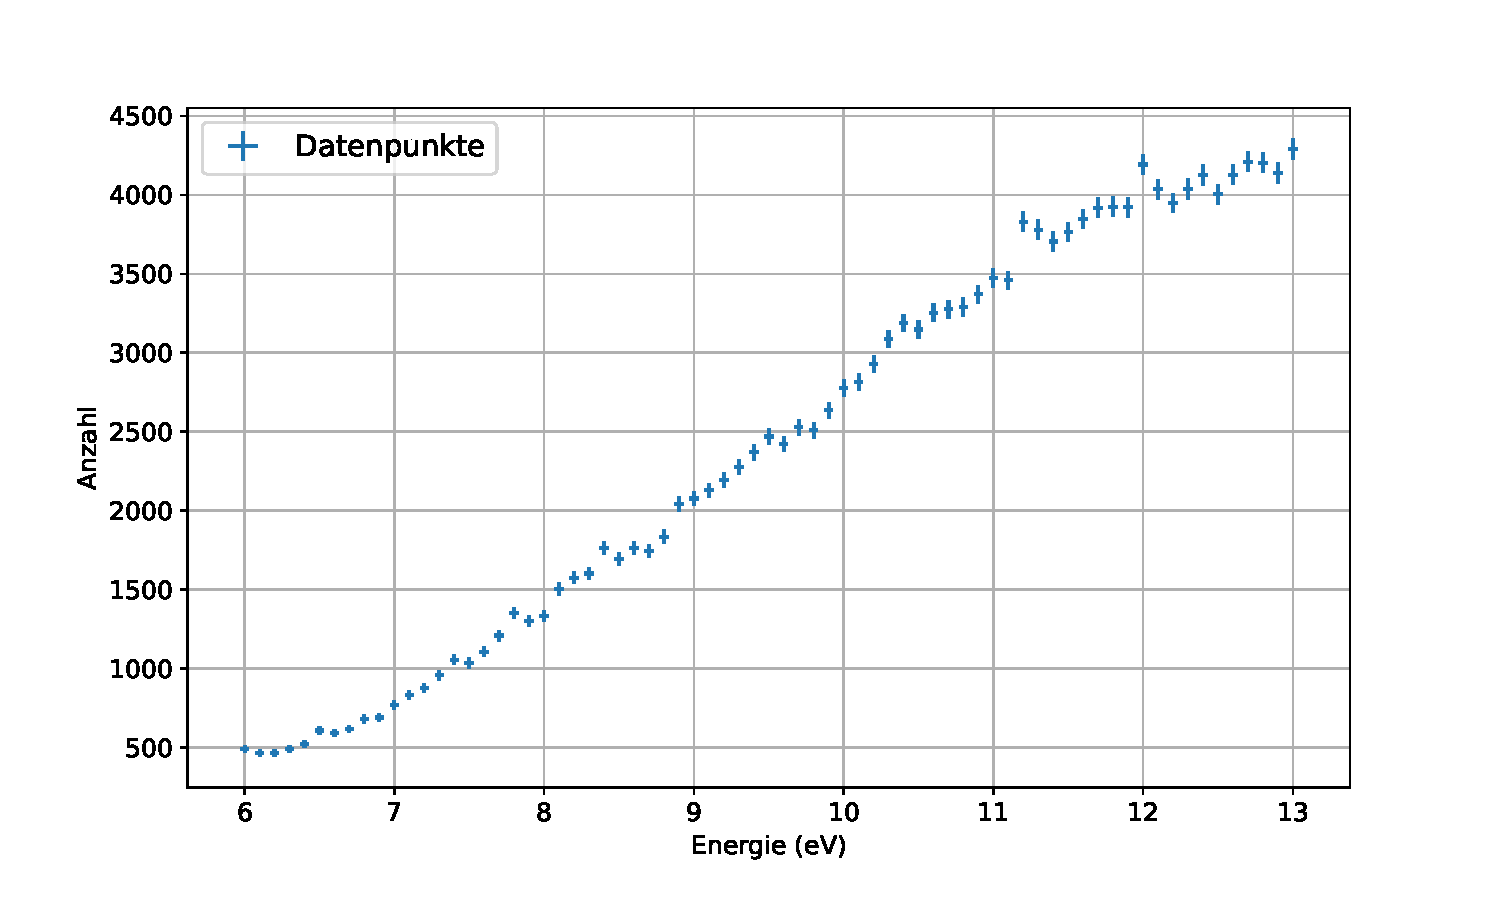
\includegraphics[width=0.85\textwidth]{plots/TiSe2.pdf}
    \caption{IPE-Spektrum der $\text{TiSe}_2$-Probe bei ca. \SI{190}{\kelvin}.}
    \label{fig_ipe_thighs2}
\end{figure}
Hier lässt sich ein annähernd linearer Verlauf erkennen.
Das Fehlen charakteristischer Peaks ist darauf zurüchzuführen, dass die Probe nicht unter die kritische Temperatur gekühlt wurde und der CDW-rückgefaltete Zustand demnach hier nicht vorliegt.

% BroFi Kommentare:

%Warum TiS2? falls das hier war, i dont recall.

%Kupfer 111 OF für Winkelkalibrierung.
%Erst irgendwas sputtern (Argon, iirc). Aceton-Gas für Zählrohr.
%Kühlen für: der manipulator ist ziemlich maissv und da ist kupferblock drin. Wenn der zu warm wird, dampft der krass aus. (500°C für 1h).
%Schnitt senkrecht durch Bandschema. Zwei Messungen, eine nahe Null (Null ja erstmal nicht bekannt) da sollte eigentlich der niederenergetische Zustand verschwinden, weil unter Fermienergie, also nicht zugängig für IPE. Oberer Zustand ist Bildladungszustand.
%Da ist dann noch so zwei Zustände drüber. Die kann man nicht unterscheiden, aber Hoffnung wäre, die zu sehen. (Oder war das schon TiS2? <- ja)

%Zweiter Tag: TiS2 rein. Leed machen. Zwischendurch immer heizen, weil Probe ist mit Selen versiegelt und das will man erst runter haben. Selen ist amorph, also einfach zu erkennen, wie viel davon im leedbild ist.
%Da dann mit warmen (gasförmigen) Stickstoff gekühlt. Oder auch dann mit flüssigem.
%Zwischendurch für die Messung auch immer runterkühlen, weil thermischer Hintergrund
%Dann wieder IPE
